\section{Aplicación de ejemplo}
(Fijarse si se puede poner en la problematica)
1)Edicion con cancelar
2)multiple cancelaciones
3)buscador
4)monitor de transacciones


\section{Nuestra herramienta: }
{\bf Aspect Pure Object } \emph{APO} es una abstracción del framework Javassist,
que nos permmite facilmente implementar un aspecto, y aplicarlo a un grupo de
objetos.
\\
Se evaluaron dos frameworks para resolver nuestro problema. Uno es Javassist y
el otro AspectJ. \cite{KiczalesHHKPG01}\\
Se utiliza Javassist porque es independiente al usuario, en cambio si utilamos
AspectJ obligamos al consummidor a cambiar la implementacion de sus objetos,
y cambiar el compilador del codigo. \\ \\ 

Utilizando esta herramienta se implementaron dos aspectos diferentes:

\begin{enumerate}

	\item {\bf Aspecto Transaccional:} Esta basado en una implementacion que
	hecha por Nicolás Passerini y Javier Fernandés.
	
	{\bf Objetivos:}
	\begin{itemize}

	  \item Obtener el concepto de transacción en el mundo de los objetos.
	  
	  \item Soprtar transacciones anidadas.
	  
	  \item Que utilize a los objetos en forma transparente.
	  
	  \item Permitir desacer los cambios. (rollback).
	  
	  \item Permitir el trabajo concurrente (nivel de insolacion.)
	  
	  \item Mantener la identidad del objeto.
	   
	\end{itemize} 
	
	Interfaz que nos provee las transacciones:
	\begin{itemize}
	  \item {\bf beginTransaction}  \emph{empezar una transacción}
	  \item {\bf commit} \emph{impactar los cambios realizados en esa transacción}
	  \item {\bf rollback} \emph{revertir los cambios realizados en esa
	  transacción}
	\end{itemize}
	
	{\bf Uso}
	\begin{itemize}
	  \item Todo el trabajo se realiza dentro de un contexto transaccional.
	  
	  \item Las modificaciones de los objetos solo pueden ser vistos dento del
	  mismo contexto, si todavia no se hizo el commit.
	   
	  \item Fuera de ese contexto, el objeto permanece sin modificar.
	  
	   \item El contexto transaccional esta asociado a thread actual.
	\end{itemize}
	
	 
	{\bf Implementación}\\
	Utilizando la programacion orientada a aspectos, intercepta todas las lecturas
	y escrituras de los fields. Insertando codigo al momento de la carga de la
	clase.
	Se remplaza el acceso al field, tanto de lectura como escritura, al
	ObjectTransactionManager.\\
	
	El contexto esta asociado a un solo tread. Implementado con variales del tipo ThreadLocal
	Soporta transacciones anidadas, donde cada transaccion hija hereda el estado
	de su padre, y al momento de hacer un commit en la sub-transaccion, su cambios
	son impactados en la transaccion padre.
	Por esta forma de implementacion, la identidad del objeto se mantiene, ya que
	el objeto no se modifica ni se clona, solo se cambia el acceso a sus fields.\\
	
	{\bf Modelo Transaccional}
	
	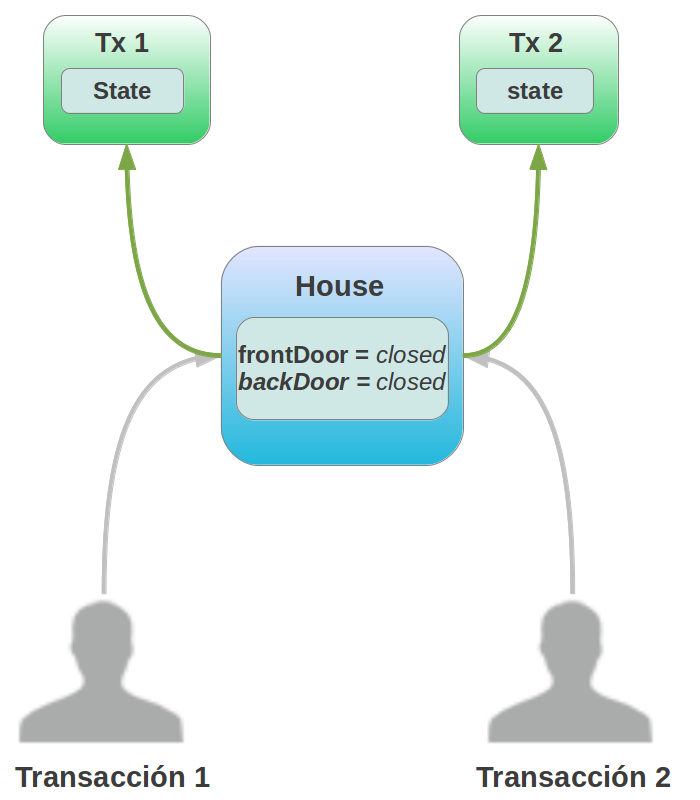
\includegraphics[width=350px, height=300px]{img/transacionalModel}
	
	{\bf Caso de uso}
	
	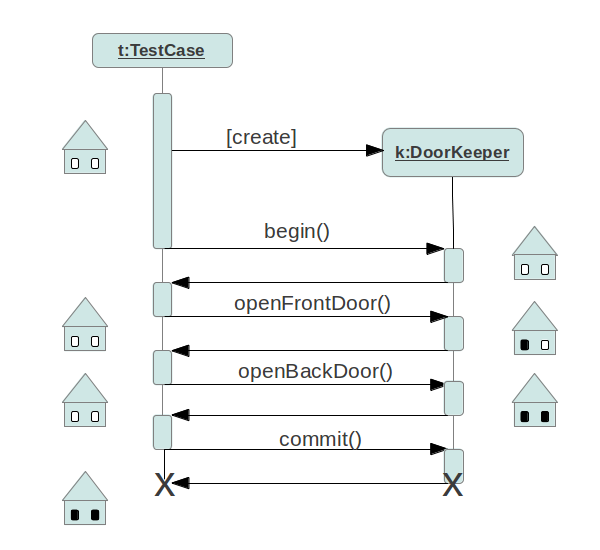
\includegraphics[width=400px, height=300px]{img/tescasePOT}
	
	{\bf Contexto de transacciones anidadas (1/8)}\\
	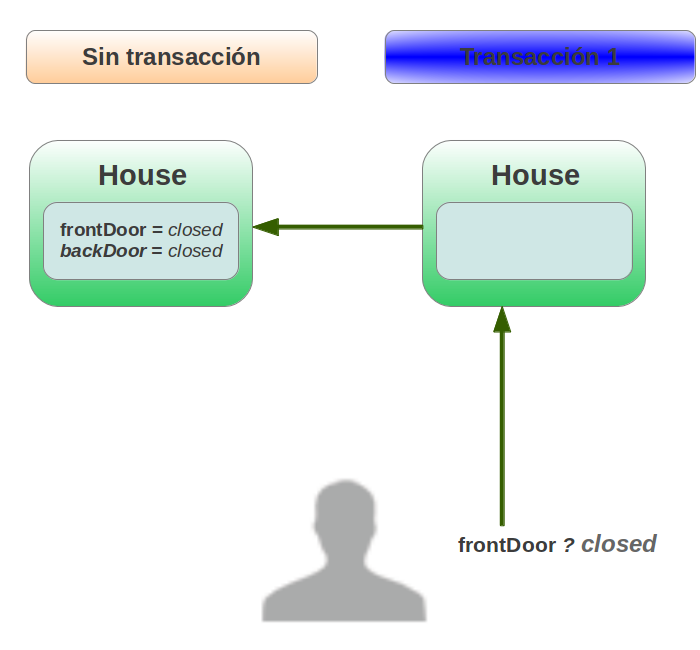
\includegraphics[width=400px, height=300px]{img/contextoAninado1}
	
	{\bf Contexto de transacciones anidadas (2/8)}\\
	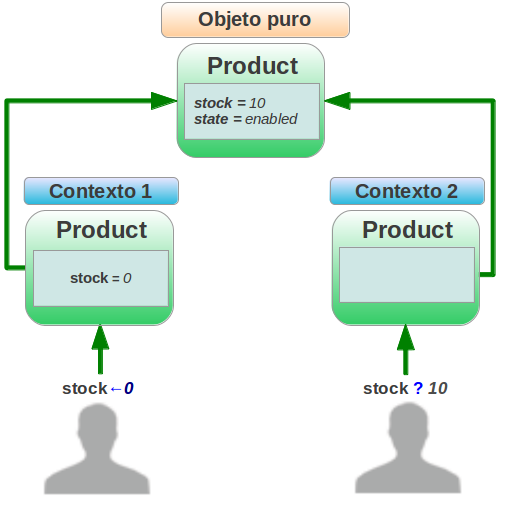
\includegraphics[width=400px, height=300px]{img/contextoAninado2}
	
	{\bf Contexto de transacciones anidadas (3/8)}\\
	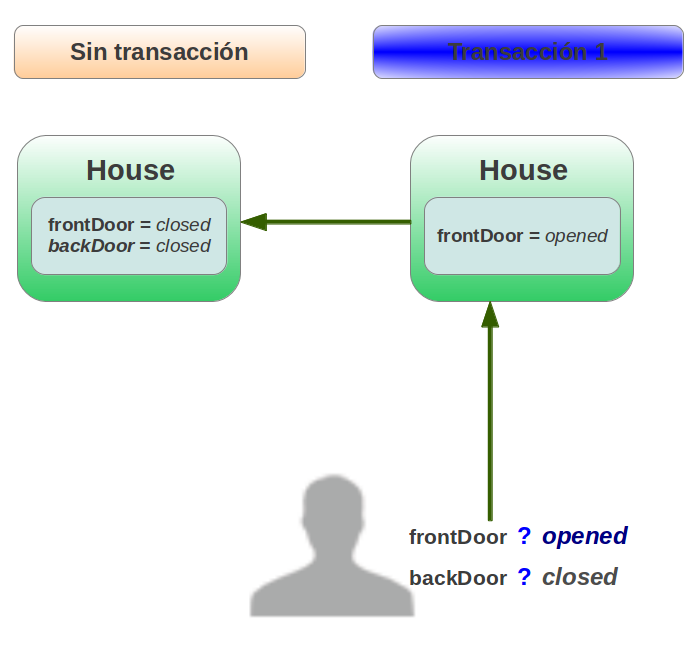
\includegraphics[width=400px, height=300px]{img/contextoAninado3}
	
	{\bf Contexto de transacciones anidadas (4/8)}\\
	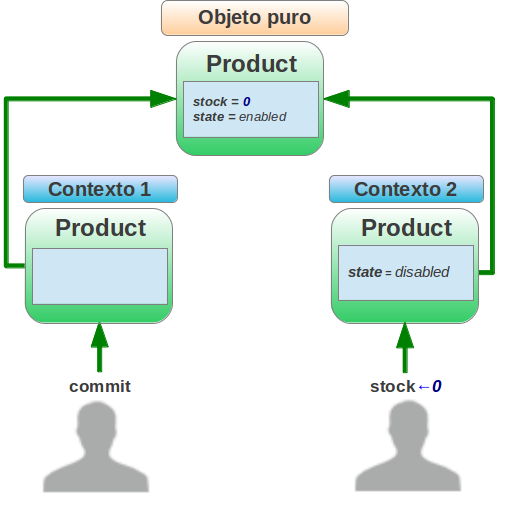
\includegraphics[width=400px, height=300px]{img/contextoAninado4}
	
	{\bf Contexto de transacciones anidadas (5/8)}\\
	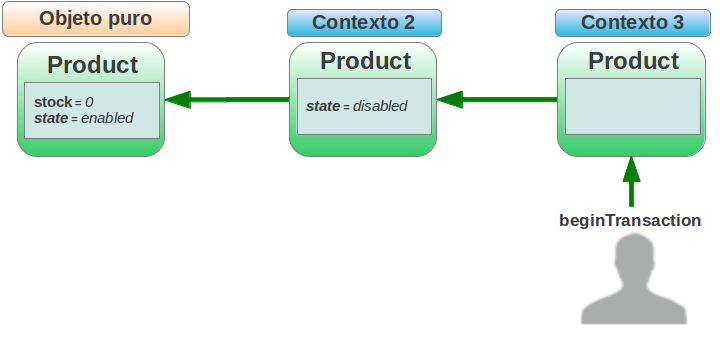
\includegraphics[width=400px, height=300px]{img/contextoAninado5}

	{\bf Contexto de transacciones anidadas (6/8)}\\
	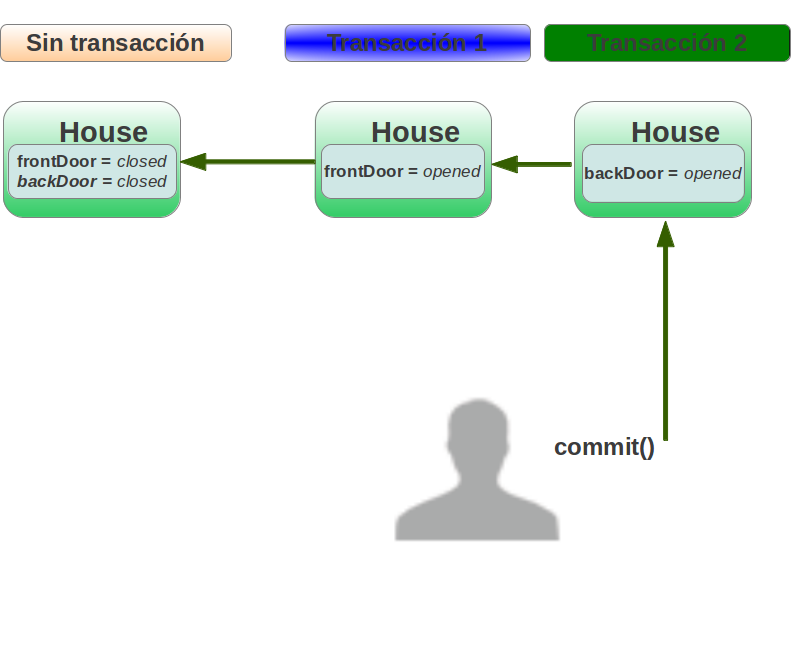
\includegraphics[width=400px, height=300px]{img/contextoAninado6}

	{\bf Contexto de transacciones anidadas (7/8)}\\
	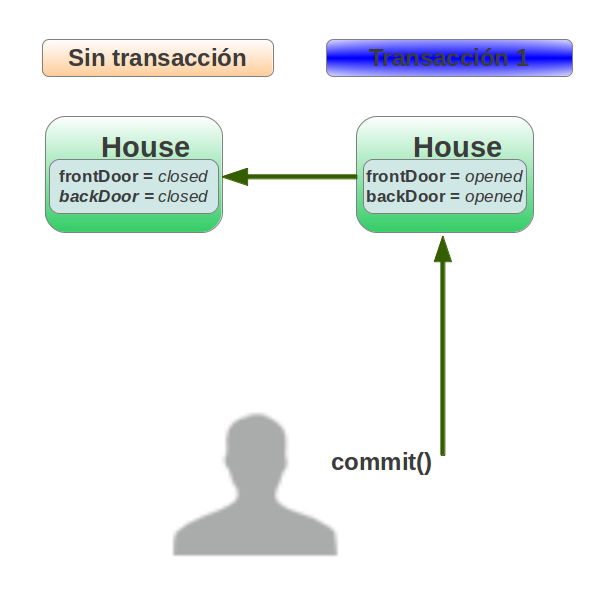
\includegraphics[width=400px, height=300px]{img/contextoAninado7}

	{\bf Contexto de transacciones anidadas (8/8)}\\
	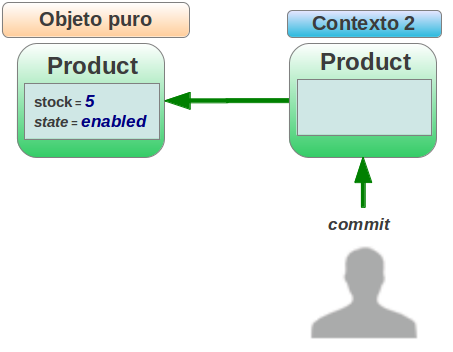
\includegraphics[width=150px, height=150px]{img/contextoAninado8}

	\item {\bf Aspecto Observable}
	El aspecto Observable tiene como objetivos:
	\begin{itemize}

	  \item Convertir un objeto de dominio en observlable, sin que el cliente lo
	  modifique.
	  
	  \item Notificar a todos los Observadores que el valor de alguna propiedad ha
	  cambiado.
	  
	\end{itemize}
		
	{\bf Implementacion}\\
	En su implementacion interna lo que hace el aspecto es agregar un field del
	tipo \emph{PropertyChangeSupport} al objeto que se va a convertir en
	Observable. Y a su vez le agrega metodos para completar su objetivo:
	El primero es el \emph{firePropertyChange} que es el que notifica a los
	Observadores que una propiedad ha cambiado.\\
	
	Luego le agregamos \emph{addPropertyChangeListener} y 
	\emph{removePropertyChangeListener} para poder agregar y remover Observadores
	para que escuchen sus cambios.
		
	 
\end{enumerate}


Integracion con el domminio
	Facil de configurar con annotations
	Poder tener una u otro aspecto 


Integración de aspectos con el Arena
	Asocio un transaccion con una ventana.
	El trabajo de los eventos va al dominio y no al arena!
	Modificar el arena para que escuche los eventos que estan solo en su
	transaccion. (contar del transaccional dialog)
	

(Mejoras al arena | utilacion de scala => fijarse donde va)
	
	
(poder hacer otra implementacion de (eventos | Swing) y utilizarlo con las
transacciones (trabajo futuro si no se llega))

Contar que esta publicado, con la licencia y blah

Test de los aspectos




--------------------
Trabajos futuros

implementar niveles de insolaicon


